\documentclass{article}

\usepackage[margin=0.5in]{geometry}
\usepackage{enumitem}
\usepackage{graphicx}
\usepackage{tikz}

\usepackage[group-separator={,}]{siunitx}

\title{2.2 Counting Lecture Problems}
\author{}
\date{}

\begin{document}
\maketitle
\section*{Problems}

\begin{enumerate}
	\item You are assigned even problems from $10$ through $40$ for tonight's 
		homework. How many problems is this?
		\vspace{3cm}
    \item Fredrick owns a rectangular plot of land that is $60$ yards long and 
    $30$ yards wide.
    \begin{enumerate}
        \item If he places a fence post at each corner and posts are placed 
            every three yards, how many fence posts will there be on each 
            side?
            \vspace{3cm}
        \item If he places a fence post at each corner and posts are placed 
            every three yards, how many fence posts will he need to enclose 
            his land?
            \vspace{3cm}
    \end{enumerate}
    \item Every student who applied for admission to a veterinary school has 
    at least one pet: $30$ have a cat, $28$ have a dog, and $26$ have 
    fish. If $13$ students have a fish and cat, $15$ students have 
    fish and dog, $11$ students have a cat and dog, and $4$ 
    students have all three, how many students applied to 
    veterinary school? 
    \begin{center}
        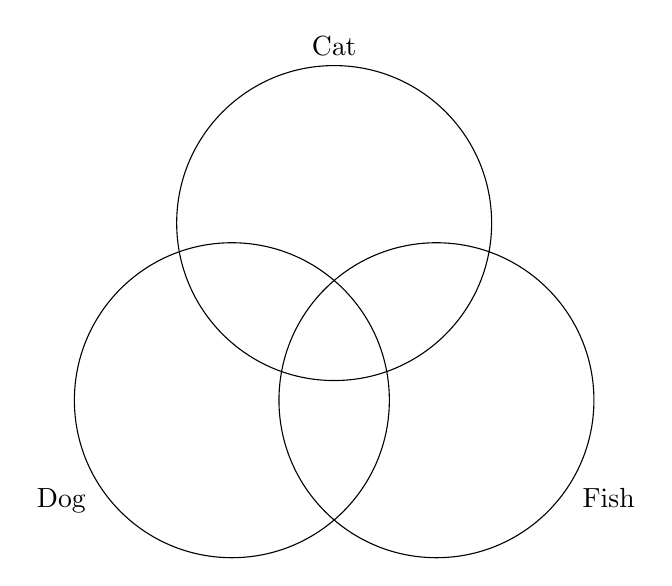
\begin{tikzpicture}
            \draw (90 : 1.5) circle (2);
            \node[above] at (90 : 3.5) {Cat};
            \draw (210 : 1.5) circle (2);
            \node[below left] at (210 : 3.5) {Dog};
            \draw (330 : 1.5) circle (2);
            \node[below right] at (330 : 3.5) {Fish};
        \end{tikzpicture}
    \end{center}
    \vspace{3cm}
    \item Akash's birthday cake is in the form of a $4 \times 4 \times 4$ inch cube.
        The cake has icing on the top and the four side faces, and no icing on the bottom.
        Suppose the cake is cut into $64$ smaller cubes, each measuring $1 \times 1 \times 1$ inch, as shown below.
        How many of the small pieces will have icing on exactly two sides?
        \begin{center}
            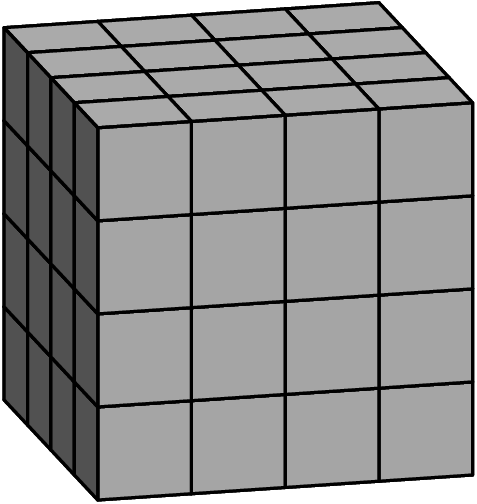
\includegraphics[scale=0.25]{cake-cube.png}
        \end{center}
        \vspace{3cm}
    \item Several couples arrive at a dinner party. Each person at the party 
		shakes the hand of every other person, not including his or her spouse.  
		If there were a total of $112$ handshakes, how many couples attended the 
		party?
\end{enumerate}
\end{document}
